\chapter{Обход графа в глубину}
\section{Множества и словари}
\noindent Задание множеств:
\begin{infanoname}
A = None \com{Пустое множество}
A = \{1, 2 'hello'\} \com{Явное перечисление элементов}
A = \seti('hello') \com{Множество букв в строке}
B = [1, 2, 1, 2]; A = \seti(B) \com{Множество из списка или любого итерируемого объекта}
\end{infanoname}
Работа с элементами множеств:
\begin{infanoname}
C = \{1, 2, 'hello'\}
\fori elem \ini \rangei(C): \com{Перебираем все элементы множества}
\tab \printi(elem)
sorted(C) \com{Список из отсортированных элементов множества}
1 \ini C \com{Проверка принадлежности}
2 \noti \ini C
A.add(3) \com{Добавление элемента}
A.remove(3) \com{Удаление элемента, который есть в множестве}
A.discard(4) \com{Удаление элемента, которого может и не быть в множестве}
A.pop() \com{Извлечение случайного элемента из множества с удалением его}
\end{infanoname}
Задание словарей
\begin{infanoname}
D = \{\} \com{Пустой словарь}
D = \{1: 'a', 2: 'b'\} \com{Явное перечисление}
D = \dicti([(1, 'a'), (2, 'b')]) \com{Словарь из списка пар элементов}
D = \dicti(\zipi([1, 2], ['a', 'b'])) \com{Словарь из итерируемого объекта, возвращающего пары\\ значений}
D = \{i: \chri(i + \ordi('a')) \fori i \ini \rangei(1, 3)\} \com{Генератор словарей}
\end{infanoname}
Работа с элементами словаря
\begin{infanoname}
\leni(D) \com{Количество элементов в словаре}
D[key] \com{Поиск по ключу, который есть в словаре}
key in D \com{Проверка принадлежности словарю}
D[key] = value \com{Установка или изменение значения}
\deli D[key] \com{Удаление ключа, который есть в словаре}
value = D.pop(key) \com{Удаление ключа вместе с возвращением значения}
value = D.pop(key, no_key_value)
key, value = D.popitem() \com{Извлечение из словаря пары (ключ, значение) с удалением ключа}
D.get(key, no_key_value) \com{Значение по ключу, no_key_value, если ключа нет}
D[key] = D.get(key, 0) + 1 \com{Самая простая реализация счетчика}
\fori key \ini D: \com{Перебираем все ключи}
\tab \printi(key, D[key])
\fori key, value \ini D.items(): \com{Перебираем все пары (ключ, значение)}
\tab \printi(kay, value)
\fori value \ini D.values(): \com{Перебор всех значений}
\tab \printi(value)
\sortedi(D) \com{Отсортированный список ключей}
\sortedi(D.values()) \com{Отсортированный список значений}
\sortedi(D.items()) \com{Отсортированный по ключу список пар (ключ, значение}
\sortedi(D.items(), \keyi = \lambdai x: x[1])
\end{infanoname}


\section{Реализация записи графа}
\begin{wrapfigure}{r}{0.25\linewidth}
		\begin{center}
			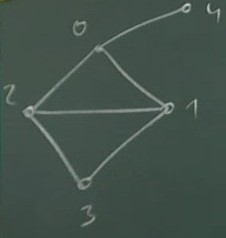
\includegraphics[width=\linewidth]{lection_18/graph1}
			\caption{Пример графа}
			\label{Fig:graph1}
		\end{center}
\end{wrapfigure}
Будем задавать граф как список ребер. Количество вершин, потом количество ребер.\\
$$5\ 6$$
После зададим ребра:
\begin{center}
0 1\\
0 2\\
1 2\\
1 3\\
2 3\\
0 4\\
\end{center}
\begin{infa}{Считывание графа как матрицы и как списка смежностей}
\ \num \defi read_graph_as_matrix():
\ \num \tab N, M = [\inti(x) \fori x \ini \inputi().split()]
\ \num \tab graph = [[0]*N \fori i \ini \rangei(N)] \com{матрица смежностей}
\ \num \tab \fori edge \ini \rangei(M):
\ \num \tab \tab a, b = [\inti(x) \fori x \ini \inputi().split()]
\ \num \tab \tab graph[a][b] = 1
\ \num \tab \tab graph[b][a] = 1
\ \num \tab \returni graph
\ \num
\num \defi print2d(A):
\num \tab \fori line \ini A:
\num \tab \tab print(*line)
\num \tab \printi()
\num
\num \defi read_graph_as_lists():
\num \tab N, M = [\inti(x) \fori x \ini \inputi().split()]
\num \tab graph = [[] \fori i \ini \rangei(N)]
\num \tab \fori edge \ini \rangei(M):
\num \tab \tab a, b = [\inti(x) \fori x \ini \inputi().split()]
\num \tab \tab graph[a].append(b)
\num \tab \tab graph[b].append(a) \com{Для ориентированного графа строка не нужна}
\num \tab \returni graph
\num
\num graph = read_graph_as_lists()
\num print2d(graph)
\end{infa}
В итоге $\texttt{read\_graph\_as\_matrix()}$ даст нам такой результат:
\begin{center}
\vspace{-1cm}
$$
\begin{matrix}
	0&1&1&0&1\\
	1&0&1&1&0\\
	1&1&0&1&0\\
	0&1&1&0&0\\
	1&0&0&0&0\\
\end{matrix}
$$
\end{center}
а $\texttt{read\_graph\_as\_lists()}$:
$$
\begin{matrix}
1&2&4\\
0&2&3\\
0&1&3\\
1&2& \\
0& & \\
\end{matrix}
$$
\section{Алгоритм обхода графа в глубину}
\subsection{Алгоритм}
Перебираем соседей по часовой стрелке. Граф считаем неориентированным.

\textbf{Основное правило: для того, чтобы пойти на праздник надо вначале позвать всех своих друзей на праздник, но только тех, кто еще не позван.}

\begin{figure}[h!]
	\centering
	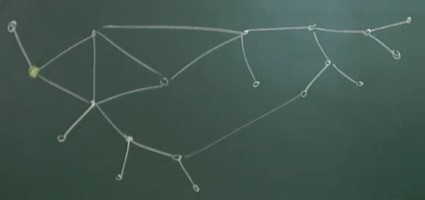
\includegraphics[width=0.5\linewidth]{lection_18/alg1}
	\caption{Граф с выбранным началом}
\end{figure}
Далее по часовой стрелке от 12 часов выбираем следующую вершину и зовём ее на праздник. Будем отмечать порядок обхода (номера показывают не индексы в графе, а просто порядок вызова).

\begin{figure}[h!]
	\centering
	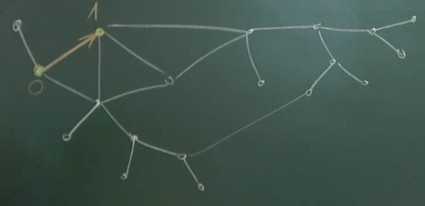
\includegraphics[width=0.5\linewidth]{lection_18/alg2}
	\caption{Точка 1 перекрашена в "серый"\ цвет}
\end{figure}

Теперь вершину 1 красим в "серый"\ цвет. 0-ой ждёт ответа от 1-го.

1-ый начинает перебирать всех своих не позванных соседей по часовой стрелке от 12 часов.
\vspace{10cm}

\begin{figure}[h!]
	\centering
	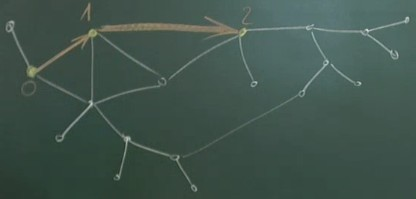
\includegraphics[width=0.5\linewidth]{lection_18/alg3}
	\caption{Точка 2 перекрашена в "серый"\ цвет}
\end{figure}

И так процесс продолжается.
\begin{figure}[h!]
	\centering
	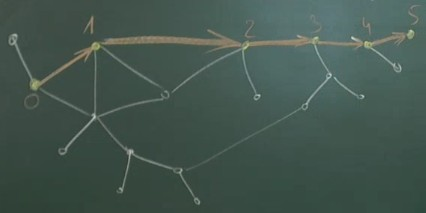
\includegraphics[width=0.5\linewidth]{lection_18/alg4}
	\caption{Точки 0-5 перекрашены в "серый"\ цвет}
\end{figure}

Теперь 5-ый перебирает всех своих соседей. Но у него только один сосед --- это 4-ый, и он уже позван. Т.о. 5-ый уже всех позвал. 5-я точка перекрашивается в "чёрный"\ цвет и идёт на праздник. 4-му возвращается от 5-го команда, что 5-ый всех позвал. Дальше 4-ый продолжает звать друзей и зовёт 6-го. 6-ая точка перекрашивается в "серый"\ цвет.

6-ой перебирает всех друзей и убеждается, что он всех позвал. Точка перекрашивается в "чёрный"\ цвет и идёт на праздник. 4-му возвращается команда, что 6-ой позвал всех друзей.

Т.о. 4-ый тоже позвал всех друзей. Точка перекрашивается в "чёрный"\ и дает команду 3-ему.

\begin{figure}[h!]
	\centering
	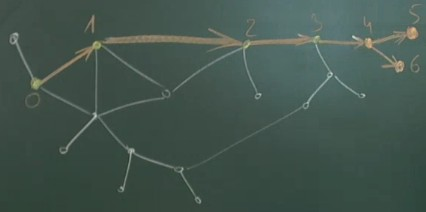
\includegraphics[width=0.5\linewidth]{lection_18/alg5}
	\caption{Точка 4 перекрашена в "чёрный"\ цвет}
\end{figure}

3-ий зовёт оставшихся.

Процесс повторяется...
\vspace{10cm}
\begin{figure}[h!]
	\centering
	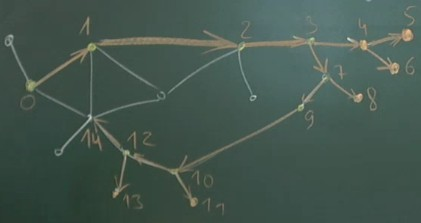
\includegraphics[width=0.5\linewidth]{lection_18/alg6}
	\caption{Дошли до 14}
\end{figure}

14-ый позвал бы 1-го, но он уже позван. Заметим, что из серой вершины мы пытаемся позвать серую вершину, что значит, что в графе есть цикл.

Т.о. 14-ый зовёт следующего по часовой стрелке. 15 точка перекрашивается в "серый". 15-му звать некого, поэтому точка перекрашивается в "чёрный"\ и дает сигнал 14-му.

\begin{figure}[h!]
	\centering
	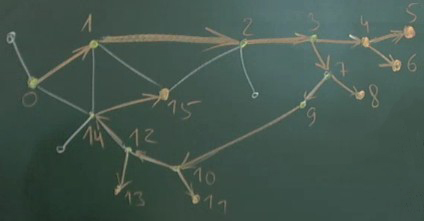
\includegraphics[width=0.5\linewidth]{lection_18/alg7}
	\caption{Прошли 15-го}
\end{figure}

14-ый продолжает звать друзей, зовёт 16-го, 16-ый возвращает сигнал 14-му.

14-му становится некого звать. Он возвращает сигнал 13-му и перекрашивается в "чёрный". 13 возвращает сигнал 12-му и т.д. до 2-го и все они идут на праздник.

\begin{figure}[h!]
	\centering
	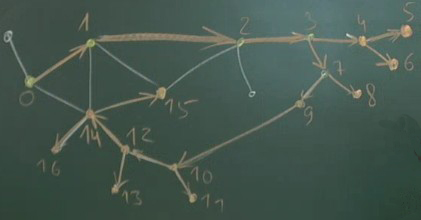
\includegraphics[width=0.5\linewidth]{lection_18/alg8}
	\caption{Длинный возврат}
\end{figure}

2-ой зовёт 17-го, ему в свою очередь звать некого, он идёт на праздник и возвращает сигнал 2-му. 2-ой тоже всех позвал. В итоге сигнал возвращается 0-му, который зовёт 18-го. В итоге, все точки перекрашены в "чёрный"\ цвет. 

\begin{figure}[h!]
	\centering
	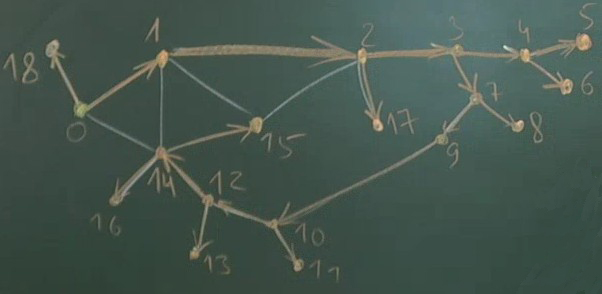
\includegraphics[width=0.5\linewidth]{lection_18/alg9}
	\caption{Все позваны}
\end{figure}

Применение обхода в глубину:
\begin{enumerate}
	\item Проверка связности графа (будем добавлять вершины в множество пройденых вершин)
	\item Выделение компонентов связности
	\item Поиск циклов (проверка ацикличности графов)
	\item Поиск компонент сильной связности орграфов (алгоритм Косарайю)
\end{enumerate}

\subsection{Реализация на Python}

\begin{infa}{Построение алгоритма}
\ \num \defi read_graph_as_lists():
\ \num \tab N, M = [\inti(x) \fori x \ini \inputi().split()]
\ \num \tab graph = [[] \fori i \ini \rangei(N)]
\ \num \tab \fori edge \ini \rangei(M):
\ \num \tab \tab a, b = [\inti(x) \fori x \ini \inputi().split()]
\ \num \tab \tab graph[a].append(b)
\ \num \tab \tab graph[b].append(a)
\ \num \tab \returni graph
\ \num 
\num \defi call_all_friends(me, friends, already_called = \Nonei):
\num \tab \ifi already_called \isi \Nonei:
\num \tab \tab already_called = \seti()
\num \tab {\color{grey}""" Правило: тебя позвали на праздник, но пойти можно только тогда, когда\\ \phantom{12 \tab \tab """}позовешь всех своих еще не позванных друзей \\\phantom{12 \tab \tab}"""}
\num \tab already_called.add(me)
\num \tab \fori friend \ini friends[me]:
\num \tab \tab \ifi friend \noti \ini already_called:
\num \tab \tab \tab \printi(friend, 'был позван на праздник')
\num \tab \tab \tab call_all_friends(friend, friends, already_called)
\num \tab \tab \tab \printi(friend, 'пошел на праздник')
\num
\num graph = read_graph_as_lists()
\num call_all_frineds(0, graph)
\end{infa}
Запишем теперь более строго:
\begin{infa}{Реализация алгоритма обхода графа в глубину}
\ \num \defi dfs(vertex, graph, used = \Nonei): \com{Depth-first search}
\ \num \tab \ifi used \isi \Nonei:
\ \num \tab \tab used = \seti()
\ \num \tab used.add(vertex)
\ \num \tab \fori neighbour \ini graph[vertex]:
\ \num \tab \tab \ifi neighbour \noti \ini used:
\ \num \tab \tab \tab dfs(neighbour, graph, used) 
\ \num
\ \num graph = read_graph_as_lists()
\num used = \seti()
\num number_of_components = 0
\num \fori vertex \ini \rangei(\leni(graph)): \com{Подсчет компонент связности}
\num \tab \ifi vertex \noti \ini used:
\num \tab \tab dfs(vertex, graph, used)
\num \tab \tab number_of_components += 1
\num
\num \printi('Количество компонент связности:', number_of_components)
\end{infa}
\section{Дерево}
Дерево --- связный граф, в котором
\begin{enumerate}
	\item Нет простых циклов
	\item От a к b только один путь
	\item $N_{\text{вершин}}=M_{\text{ребер}}+1$
\end{enumerate}

Ориентированное дерево --- ациклический орграф, в котором только одна вершина имеет нулевую степень захода (корень).
Вершины с нулевой степенью исхода называются "листья". Остальные --- узлы ветвления. Для корневого дерева можно ввести уровень узла --- длина пути от корня до вершины (уровень иерархии).

У любого связного графа есть подграф, являющийся деревом и содержащий все исходные вершины.

Вершина сама по себе тоже является деревом.

Остовное дерево --- пограф исходного графа, в котором выброшено максимальное количество ребер так, чтобы связность еще сохранилась. Обход графа в глубину позволяет построить одно из остовных деревьев.

Свойства:
\begin{itemize}
	\item Дерево не имеет кратных ребер и петель
	\item Граф является деревом $\Leftrightarrow$ когда любые две различные вершины можно соединить  единственным простым путем (простой цепью).
	\item Любое дерево однозначно определяется расстояниями между его концевыми вершинами со степенью 1 (длиной наименьшей цепи).
	\item Любое дерево, множество вершин которого более чем счетное является планарным графом.
\end{itemize}

Шарнир --- вершина, при удалении которой количество компонент связности увеличивается.

\begin{wrapfigure}{r}{0.2\linewidth}
	\begin{center}
		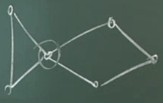
\includegraphics[width=\linewidth]{lection_18/sharnir}
		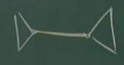
\includegraphics[width=\linewidth]{lection_18/most}
		\caption{Шарнир и мост}
		\label{Fig:sharnir}
		\vspace{-4cm}
	\end{center}
\end{wrapfigure}

Мост --- ребро, при удалении которого количество компонент связности увеличивается. Такие ребра еще известны как разрезающие ребра или перешейки.

У дерева любая вершина является шарниром, а любое ребро мостом.


\section{Алгоритм Косарайю}
Задача: поиск сильно связной компоненты орграфа. Возьмем такой орграф. В нем будет 1 слабая компонента.
\vspace{1.2cm}
\begin{figure}[h!]
	\centering
	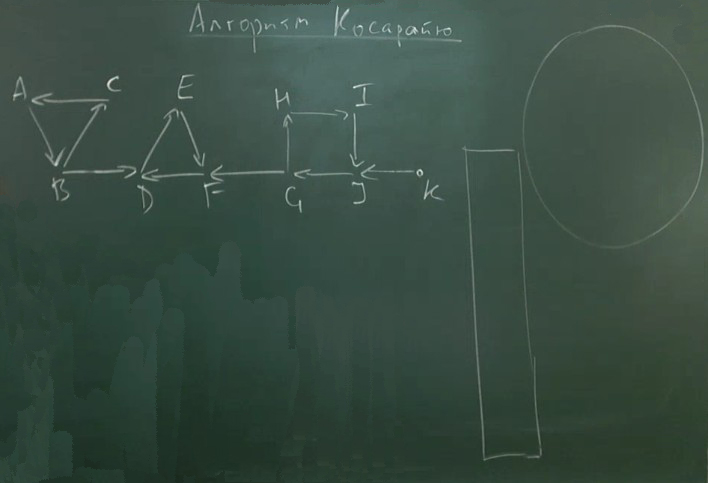
\includegraphics[width=0.8\linewidth]{lection_18/kos1}
	\caption{Орграф}
\end{figure}

Запустим обход в глубину. Пусть будет множество вершин, которых мы уже использовали, и список вершин в порядке обхода (типа как стек).

Начнем с вершины A. Из A вызываем B. Они оказываются в множестве использованных вершин, также заполняется стек вызванных вершин. Далее вызовем вершину D (не принципиально D или C), добавим ее в множество и стек аналогично. Далее вызовем E, потом F. После происходит откат, и мы вызываем вершину C. Дальше выбираем любую вершину, которую не использовали. Пусть это будет G. Потом вызываем H, I, J. Остается вершина K, она становится последней.
\vspace{10cm}
\begin{figure}[h!]
	\centering
	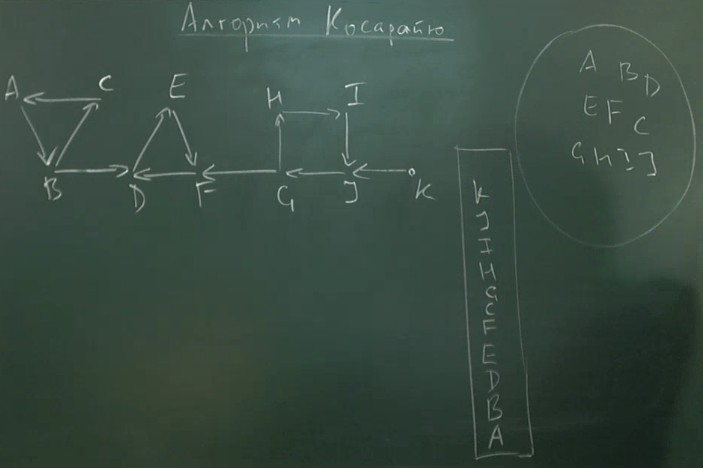
\includegraphics[width=0.8\linewidth]{lection_18/kos2}
	\caption{После прохождения по графу}
\end{figure}

Далее мы разворачиваем наш граф, т.е. меняем все направления. А теперь от верхней вершины в стеке запустим обход в глубину на обращенном графе.

\begin{figure}[h!]
	\centering
	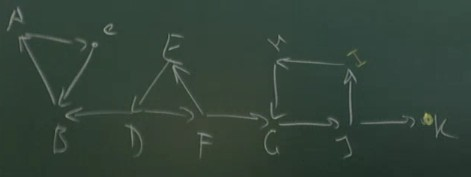
\includegraphics[width=0.5\linewidth]{lection_18/kos3}
	\caption{Обращенный граф}
\end{figure}

Но от K дойти никуда нельзя. Это и есть сильная компонента. K добавляем в новое множество использованных вершин. 

Дальше начинаем обход с вершины I, т.е. I--->H--->G--->J. Их добавляем в множество использованных и стираем из стека. Дальше идти опять некуда. Значит, это вторая сильная компонента.

Переходим к вершине C. Выполняем обход: C--->B--->A. Их добавляем в множество использованных и стираем из стека. Дальше идти некуда. Т.о. это еще одна компонента сильной связности.

Переходим к вершине F. В G уже не идем т.к. она использована. Выполняем обход F--->E--->D. Их добавляем в множество использованных и стираем из стека. Дальше идти некуда. Т.о. это еще одна компонента сильной связности.

В итоге получилось 4 компонент сильной связности.

Примечание: не принципиально, оборачивать ли граф сначала или потом (по \href{https://ru.wikipedia.org/wiki/%D0%90%D0%BB%D0%B3%D0%BE%D1%80%D0%B8%D1%82%D0%BC_%D0%9A%D0%BE%D1%81%D0%B0%D1%80%D0%B0%D0%B9%D1%8E}{википедии} сначала нужно развернуть граф).